\documentclass{beamer}
\usepackage{tikz}
\usepackage{amsmath}
\usepackage{verbatim} 
\usepackage{svg}
\usepackage{listings}
\usepackage{courier}
\usetikzlibrary {decorations}
\usetikzlibrary{decorations.pathreplacing}
\usepackage[european,s traightvoltages, RPvoltages, americaninductors]{circuitikz}
\tikzset{every picture/.style={line width=0.2mm}}
\usetheme{metropolis}           % Use metropolis theme
\title{A probabilistic electrical simulator}
\date{February 01, 2024}
\author{Jonas Bodingbauer}

\institute{}
\lstdefinelanguage{Julia}%
  {morekeywords={abstract,break,case,catch,const,continue,do,else,elseif,%
      end,export,false,for,function,immutable,import,importall,if,in,%
      macro,module,otherwise,quote,return,switch,true,try,typealias,%
      using,while},%
   sensitive=true,%
   alsoother={$},%
   morecomment=[l]\#,%
   morecomment=[n]{\#=}{=\#},%
   morestring=[s]{"}{"},%
   morestring=[m]{'}{'},%
}[keywords,comments,strings]%

\lstset{
  language         = Julia,
  basicstyle       = \ttfamily\scriptsize,
  keywordstyle     = \bfseries\color{blue},
  stringstyle      = \color{magenta},
  commentstyle     = \color{ForestGreen},
  showstringspaces = false,
}

\begin{document}
  \maketitle

  \begin{frame}
    \frametitle{Electrical Circuit: Voltage divider}
    \begin{figure}
      \centering
        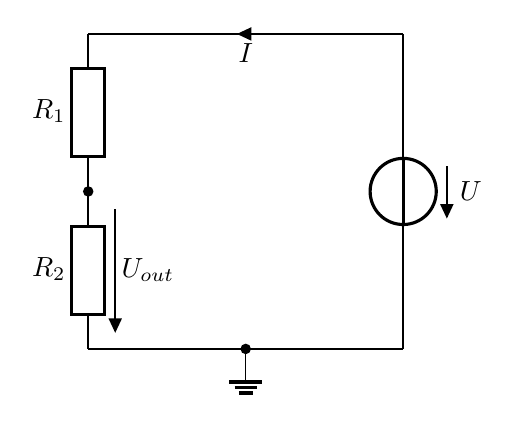
\begin{tikzpicture}
          \draw (4,4) to [short, i=$I$] (0,4);
          \draw  (0,0) to [R=$R_2$, v=$U_{out}$, -*] (0,2) to [R=$R_1$] (0,4);
          \draw (0,0) to [short] (4,0);
          \draw (4,4) to [V=$U$] (4,0);
          \draw (2,0) to [short, -*] (2,0) node[ground]{}; 
        \end{tikzpicture}
    \end{figure}

    \[U_{out} = U \frac{R_2}{R_1 + R_2}\]
  \end{frame}

  \begin{frame}
    \frametitle{Idea}
    \begin{itemize}[<+->]
      \item \emph{Components} in a circuit: \emph{expected value} and a \emph{tolerance}.  \\ \only<4->{$\rightarrow$ \textbf{Priors}}
      \item \emph{Circuit} gets input $\rightarrow$ response 
      \item The \emph{response} is a random variable, which can be described by a probability distribution. \only<4->{$\rightarrow$ \textbf{Observed}}
      \only<5>{\item  Even more randomness! Noise of devices, Noise of measurement instruments, offsets, ...} 
    \end{itemize}
  \end{frame}

  
  \begin{frame}
    \frametitle{Electrical Simulations}
    \begin{itemize}
      \item \only<1>{DC Analysis} \only<2>{\textbf{DC Analysis}}
      \item \only<1>{AC Analysis (treat everything as a linear component)} \only<2>{\textbf{AC Analysis} (treat everything as a linear component)}
      \item \only<1>{DC Analysis with nonlinearity (e.g. diodes)} \only<2>{\textbf{DC Analysis with nonlinearity} DC Analysis with nonlinearity (e.g. diodes)}
      \item Transient Analysis
      \item Lots more... 
    \end{itemize}
  \end{frame}
  \begin{frame}
    \frametitle{Finally, some modelling!}
    \[ 
    \underbrace{\begin{bmatrix}
      \mathbf{Y'} & \mathbf{B}\\
      \mathbf{C} & \mathbf{D}
    \end{bmatrix} }_{Y}
    \cdot
    \underbrace{\begin{bmatrix}
      \vec{\varphi}\\
      \vec{I}
    \end{bmatrix}}_{x}
    =
    \underbrace{\begin{bmatrix}
      \vec{J}\\
      \vec{E}
    \end{bmatrix}}_{F}
    \]
    \pause
    AC-Case: Domain changes to complex numbers (Fourier transform)

    \pause
    Nonlinear Case: Newton-Raphson Fixpoint iteration
    \[ 
      \mathbf{Y}(\vec{x}_i) \cdot \vec{x}_{i+1} = -\mathbf{F}(\vec{x}_i) + \mathbf{Y}(\vec{x}_i) \cdot \vec{x}_i
    \]
    
  \end{frame}

  \begin{frame}[fragile]
    \frametitle{Program flow}
    \begin{enumerate}
      \item Read SPICE - like file
    \begin{center}

    \begin{columns}
      \begin{column}{0.33\textwidth}
        voltagediv.cir:

        \begin{verbatim}
V1 0 in DC 2 
R3 in 2 11.72
R1 2 3 1.2k
R2 3 0 1.8k
        \end{verbatim}
      \end{column}
      \begin{column}{0.33\textwidth}
        voltagediv.tol:
        \begin{verbatim}
R3 0.1%
R1 5%
R2 5%
        \end{verbatim}
      \end{column}
    \end{columns}
  \end{center}
  \item Determine the matrix size
  \item Read observed data from file(s)
  \item Run inference using the simulator as a model
  \end{enumerate}

  \end{frame}
  
  \begin{frame}
    \frametitle{Measurements}
    \begin{columns}
      \begin{column}{0.5\textwidth}
        \includegraphics[width=\textwidth]{images/circuit.jpeg}
      \end{column}
      \begin{column}{0.5\textwidth}
        \includegraphics[width=\textwidth]{images/osci.jpeg}
      \end{column}
    \end{columns}
    \begin{center}
      \includegraphics[width=.33\textwidth]{images/realvalue.jpeg}
    \end{center}
  \end{frame}
  \begin{frame}{First example extended}
    \begin{columns}
      \begin{column}{0.3\textwidth}
        \begin{figure}
          \centering
            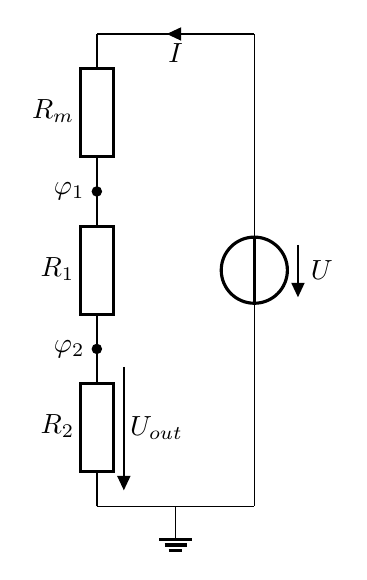
\begin{tikzpicture}
              \draw (2,6) to [short, i=$I$] (0,6);
              \draw  (0,0) to [R=$R_2$, v=$U_{out}$] (0,2) to [R=$R_1$] (0,4) to [R=$R_m$] (0,6);
              \draw (0,0) to [short] (2,0);
              \draw (2,6) to [V=$U$] (2,0);
              \draw (1,0) to (1,0) node[ground]{}; 
              \draw (0,2) node[xshift=-1em]{$\varphi_2$};
              \draw (0,4) node[xshift=-1em]{$\varphi_1$};
              \draw (0,2) node[circ]{};
              \draw (0,4) node[circ]{};
            \end{tikzpicture}
        \end{figure}
      \end{column}
      \begin{column}{.7\textwidth}
        \begin{itemize}
          \item $R_m$ is an additional (precision) resistor for measuring the current.
          \item $\varphi_1$ and $\varphi_2$ are potentials 
          \item Priors:
          \begin{itemize}
            \item  $R_1$, $R_2$, normally distributed around nominal value.
            \item $U_{offset_{1}}$, $U_{offset_{2}}$ normally distributed around 0.
            \item $U_{noise_{1}}$, $U_{noise_{2}}$ uniformly distributed $[0,0.1]V$.
          \end{itemize}
          \item Observed: $\varphi_1$, $\varphi_2$
        \end{itemize}
      \end{column}
    \end{columns}
  \end{frame}
  \begin{frame}
    \frametitle{Results}
    \includesvg[width=\textwidth]{images/divider_data.svg}
  \end{frame}
  \begin{frame}
    \frametitle{Glorified linear regression?}
    \begin{center}
      \only<1>{\includesvg[height=.8\textheight]{images/divider_sampling.svg}}
      \only<2>{\includesvg[height=.8\textheight]{images/divider_sampling_more.svg}}
      \only<3>{\includesvg[height=.8\textheight]{images/divider_sampling_hexbin.svg}}
      \only<4>{
      \begin{tabular}{cccc}
        \textbf{Component}  & \textbf{Nominal Value} & \textbf{"True" Value} &\textbf{MAP-Estimate} \\
        $R_1$          & $1.2\,\text{k}\Omega$ & $1.176\,\text{k}\Omega$ & $1.186\,\text{k}\Omega$\\
        $R_2$          & $1.8\,\text{k}\Omega$ & $1.784\,\text{k}\Omega$ & $1.776\,\text{k}\Omega$\\
        $R_3$          & $11.72\Omega$         & $11.72\Omega$ & $11.72\Omega$           \\
        $U_{offset_1}$ & $?$                   & ? & $-0.059\text{V}$       \\
        $U_{offset_2}$ & $?$                   & ? & $-0.026\text{V}$       \\
        $U_{noise_1}$  & $?$                   & ? &  $0.2   m\text{V}$     \\
        $U_{noise_2}$  & $?$                   & ? &  $10^{-5}\text{V}$      \\
      \end{tabular}
    }
    \end{center}
    
  \end{frame}
  
  \begin{frame}{A more complex circuit}
    \begin{circuitikz}
        \draw
        (7,-.5) node [op amp, yscale=-1] (opamp) {}
        (-1,0) node [left] {$U_{in}$} (-1,0) to [R, l=$R_{measure}$, o-] (1,0) to [R, l=$R_1$] (3,0)
        to [R, l=$R_2$, *-] (5,0)
        (1,-0.3) node {$\varphi_1$}
        (3,-0.3) node {$\varphi_2$}
        (5,0.3) node {$\varphi_3$}
        (8.5,-2) node {$\varphi_4$}
        (8.5,0) node {$\varphi_5$}
        (5,0) to [C, l_=$C_{1}$, *-] (5,-2) node [ground] {}
        (5,0) to [short] (opamp.+)
        (opamp.out) |- (8,1) to [C, l_=$C_{2}$] (3,1) to [short] (3,0)
        (opamp.out) to [short, *-o] (9,-0.5) node [right] {$U_{out}$}
        (opamp.out) to [R, l_=$R_3$, -*] (8.2,-2) to [short] (5.8,-2) to [short] (opamp.-) 
        (8.2,-2) to [R, l_=$R_4$] (8.2,-3.5) node [ground] {}
        ;
  \end{circuitikz}
  \end{frame}
    
  \begin{frame}{Frequency Response}
    \includesvg[width=\textwidth]{images/sallenkeyx_data.svg}
  \end{frame}

  \begin{frame}
    \begin{center}
      \includesvg[height=\textheight]{images/pairplot_sallenkey.svg}
    \end{center}
  \end{frame}

  \begin{frame}
    \begin{center}
      \includesvg[height=\textheight]{images/pairplot_sallenkey_vs_prior.svg}
    \end{center}
  \end{frame}

  \begin{frame}{Results}
    Obtained with three measured potentials: $\varphi_1$, $\varphi_2$, $\varphi_5$.

    \begin{tabular}{crrr}
      \textbf{Component}  & \textbf{Nominal Value} & \textbf{"True" Value} &\textbf{MAP-Estimate} \\
      $R_1$          & $100\,\text{k}\Omega$ & $100.09\,\text{k}\Omega$ & $100.08\,\text{k}\Omega$\\
      $R_2$          & $100\,\text{k}\Omega$ & $99.97\,\text{k}\Omega$  & $98.6\,\text{k}\Omega$\\
      $R_3$          & $150\,\text{k}\Omega$ & $149.5\,\text{k}\Omega$  & $151.2\,\text{k}\Omega$           \\
      $R_4$          & $100\,\text{k}\Omega$ & $100.06\,\text{k}\Omega$ & $99.19\Omega$           \\
      $C_1$          & $3.3\,\text{nF}$      & $2.75\,\text{nF}$        & $2.73\,\text{nF}$           \\
      $C_2$          & $3.3\,\text{nF}$      & $3.33\,\text{nF}$        & $3.32\,\text{nF}$           \\
    \end{tabular}
  \end{frame}


  \begin{frame}{Inference}
    \begin{itemize}
      \item Turing NUTS sampler performs really well
      \item Also tried other samplers (SMC, PG, Gibbs) but they did not work reasonably well (without further tuning) 
      \item ADVI works wonders for this application (MAP estimate in seconds)
      \item Choice of priors is important: often, there output depends on a ratio of variables $\rightarrow$ scaled variables might be equally likely.
    \end{itemize}
  \end{frame}

  \begin{frame}{Normal distributed priors}
    \includesvg[width=\textwidth]{images/divider_sampling_hexbin.svg}
  \end{frame}
  
  \begin{frame}{Uniform priors}
    \includesvg[width=\textwidth]{images/divider_sampling_uniform.svg}
  \end{frame}


  \begin{frame}{Challenges}
    \begin{itemize}[<+->]
      \item Getting Automatic Differentiation to work was quite a hassle (types...) \pause
      \item Big range of values (e.g. $10^{-12} - 10^{6}$) $\rightarrow$ does not seem to work nicely with NUTS
      \begin{itemize}
        \item Fixed by scaling variables
        \item Logarithmic frequency response (standard)
      \end{itemize}
      \item Hard to know if results are actually reasonable if you don't know the "true" values
    \end{itemize} 
  \end{frame}

  \begin{frame}
    \frametitle{Conclusion}
    \begin{itemize}
      \item \textbf{It works!}
      \item Modelling needs to account many things to be realistic (Measurement device offsets, noise, parasitics, ...)
      \item The nonlinear system suffers from convergence issues with some parameters explored by inference
      \item More components: Transistors (BJT, MOSFETs, ...)
      \item Transient analysis
    \end{itemize}
  \end{frame}


  \begin{frame}
    \begin{center}
      \Huge{Thank you for your attention! \\ Questions?}
      \begin{center}
        \includegraphics[width=.3\textwidth]{images/qrcode.png}
        
        \normalsize git: https://github.com/Caesiumhydroxid/SBICE
      \end{center}
      
    \end{center}
  \end{frame}

  \begin{frame}{Nonlinear Diode}
    \includesvg[width=\textwidth]{images/diode_inference.svg}
  \end{frame}


  \begin{frame}[fragile]{DC Analysis Model}
    \begin{lstlisting}[numbers=left]
@model function dcanalysis(...)
  for e in keys(tolerances) ...
      elementsR[e].R ~ Normal(elements[e].R, 
                  elements[e].R * tolerances[e]) 
  end
  offsets ~ MvNormal(zeros(observedNodeIndicesLength), 
                    diagm(0.01.*ones(observedNodeIndicesLength)))
  for i in 1:observedNodeIndicesLength
      noise[i]   ~ Uniform(0, 0.01)
  end
  A,RHS = assembleMatrixAndRhs(elementsR,nodes,type)
  Ainv = inv(A)
  for i in 1:amountOfMeasurements
      RHS[nodes[elementsR["V1"].name]-1] = -voltages[i]
      res = Ainv*RHS
      results[i,:] = res[observedNodeIndices] 
  end
  for (i,col) in enumerate(eachcol(results))
      measurementMatrix[:,i] ~ MvNormal(col.+offsets[i], 
              diagm(noise[i]*ones(amountOfMeasurements)))
  end
end
    \end{lstlisting}
  \end{frame}

  \begin{frame}[fragile]{Sallen Key Input}
    \begin{columns}
      \begin{column}{.3\textwidth}
        \begin{verbatim}
V1 0 in AC 1
R5 in 1 1.484k
R1 1 2 100k
R2 2 3 100k
C1 2 out 3.3n
C2 3 0 3.3n
R3 out 4 150k
R4 4 0 100k
O1 3 4 out 0 1e5
        \end{verbatim}
      \end{column}
      \begin{column}{.3\textwidth}
        \begin{verbatim}
R5 0.001%
R1 0.5%
R2 0.5%
R3 0.5%
R4 0.5%
C1 40%
C2 40%
        \end{verbatim}
      \end{column}
    \end{columns}
  \end{frame}
  \begin{frame}[fragile]{Sallen Key Measurements}
    \scriptsize
    \begin{center}
      

    \begin{verbatim}
in Sa,Frequency in Hz,Gain in dB,Phase in °,Amplitude in Vpp
1.00E+00,1.000E+01,-2.426E-02,2.693E-03,2.500E+00
2.00E+00,1.023E+01,-2.448E-02,3.685E-03,2.500E+00
3.00E+00,1.047E+01,-2.481E-02,6.256E-04,2.500E+00
4.00E+00,1.072E+01,-2.359E-02,1.049E-02,2.500E+00
5.00E+00,1.096E+01,-2.475E-02,1.010E-02,2.500E+00
6.00E+00,1.122E+01,-2.326E-02,4.135E-03,2.500E+00
7.00E+00,1.148E+01,-2.272E-02,1.164E-02,2.500E+00
8.00E+00,1.175E+01,-2.387E-02,-7.126E-03,2.500E+00
9.00E+00,1.202E+01,-2.171E-02,1.350E-03,2.500E+00
...
    \end{verbatim}
  \end{center}
  \end{frame}
\end{document}